\documentclass[12pt,a4paper,Flow]{report}
\usepackage[left=2.8cm,right=2.8cm,top=2.5cm,bottom=2cm]{geometry}
\usepackage[BoldFont]{xeCJK}
\usepackage{xcolor}
\usepackage{graphicx}
\usepackage{colortbl}
\usepackage{float}
\usepackage{indentfirst}
\usepackage{fancyhdr}
\usepackage[toc,header,title]{appendix}
\usepackage{listings}
\usepackage{tikz}
\defaultfontfeatures{Mapping=tex-text}
\definecolor{llgray}{rgb}{0.9,0.9,0.9}
\lstloadlanguages{[ansi]c}
\lstset{
  language=python,tabsize=4,keepspaces=true,
  xleftmargin=2em,xrightmargin=2em,aboveskip=1em,
  frame=none,
  commentstyle=\color{red}\itshape, % blue comments
  keywordstyle=\color{blue}\bfseries,
  backgroundcolor=\color{llgray},
  breakindent=22pt,
  numbers=left,stepnumber=1,numberstyle=\tiny,
  basicstyle=\footnotesize,
  showspaces=false,
  showstringspaces=false, % show explicit string spaces
  flexiblecolumns=false,%true,
  breaklines=true,breakautoindent=true,breakindent=4em,
  escapeinside={/*@}{@*/}
}
\usepackage[a4paper,CJKbookmarks,bookmarks=true,bookmarksopen=true]{hyperref}
\hypersetup{
  pdftitle={},
  pdfauthor={Wang Pei},
  pdfkeywords={},
  bookmarksnumbered,
  breaklinks=true,
  pdfview=FitV,       % Or try pdfstartview={FitV}, This lead to uncorre
  urlcolor=cyan,
  colorlinks=true,
  citecolor=magenta,          %citeref's color
  linkcolor=blue,
}
\usepackage{titlesec}
\titleformat{\chapter}{\centering\huge}{\textbf{第}\thechapter{} \textbf{章}}{1em}{\textbf}
\renewcommand\contentsname{目录}
\renewcommand{\appendixpagename}{附录}
\renewcommand{\appendixname}{附录}
\setmainfont{DejaVu Sans}
\setCJKmainfont[BoldFont=WenQuanYi Micro Hei]{SimSun}

\begin{document}
\title{\textbf{编译实习——minicc编译器\\实习报告}}
\author{张番栋 00848180\\刘澜涛 00848200\\王 沛 00848205}
\date{}
\maketitle
\tableofcontents
\newpage
\chapter{实习内容}
实习的内容是以C语言编写一个以C语言子集(称为MiniC)为源程序,目标机为UniCore2体系结构的编译器。报告后面的篇幅中,均称实习中编写的编译器为minicc。MiniC的语法与C语言基本相同,比较重要的区别是不支持除法、浮点计算、多重指针和高维数组。\\
\indent 实习对minicc的基本要求是,可以对给定的源程序进行语法和语义上的正确性检查并能够输出正确的汇编程序代码,最终与体系结构实习所完成的模拟器协同工作。这一过程需要的预处理器、库以及二进制工具由外部提供。
\chapter{编译器前端}
minicc前端的任务有
\begin{enumerate}
\item 针对源程序进行词法、语法分析。
\item 在语法分析的过程中构建抽象语法树、建立符号表。
\item 针对语法树进行语义检查,包括类型检查与左值存在性检查。
\item 生成中间代码。
\end{enumerate}
下面对各项工作进行详细说明。
\newpage
\section{词法、语法分析}
minic的词法和语法分析部分代码由flex和bison辅助生成。\\
\indent 就词法分析而言,由于MiniC的文法并没有对源程序中字符、字符串的形式做规定,因此在实现时,我们只支持了最普通的一种,十六进制形式的字符和字符串常量并不被词法分析过程接受。\\
\indent 语法分析方面,我们对原始的MiniC文法进行了一定修改,使其支持悬空if控制流。另外通过规定运算符优先级和结合性的方式避免的文法规约时的二义性。
\section{构建抽象语法树}
\subsection{数据结构描述}
处于简化数据结构的考虑,在语法分析的过程中仅对计算语句构建抽象语法树。控制流的实现在进行文法规约时同步处理,这一点在之后还会详细说明。\\
\indent minic语法总只有一元和二元运算符,因此将语法树定义为二叉结构。源程序中一个表达式对应一棵语法树,语法树的叶节点根据词法分析过程的返回信息生成,具体类型包括三种:整型常量、字符串常量和标识符。语法树的数据结构定义如下:
\begin{lstlisting}[language=c]
struct ast
{
    /* node type */
    struct typetree * ast_typetree;
    enum operator op;
    int isleaf;
    struct ast* left;
    union
    {
        struct ast* right;    /* isleaf = 0 */
        struct leafval* val;  /* isleaf = 1 */
    };
};

enum leaftype { Iconstleaf, Sconstleaf, Idleaf };

struct leafval
{
    enum leaftype ast_leaf_type;
    union
    {
        char* sval;
        int ival;
    };
};
\end{lstlisting}
C语言的基本类型系统比较简单,因此我们主要通过union与指针相结合的方式来实现比较复杂的数据结构。这一点贯穿了整个minicc的实现。
\subsection{常量处理}
根据C语言标准,源程序中出现的字符常量全部视为整型常量,因此语法树中没有表示字符常量的结构。通过在语法分析中加入判断常量表达式的语句,minicc在构建语法树时已经将源程序中的常量表达式全部计算完毕。下面是计算常量表达式的一部分代码样例:\\
\begin{lstlisting}[language=c]
binary_expr : binary_expr "+" binary_expr  /* bnf */
{
  if(($1->isleaf && $1->val->ast_leaf_type == Iconstleaf) &&
     ($3->isleaf && $3->val->ast_leaf_type == Iconstleaf))
  {
    /* if both sub exprs are integer constants */
    $1->val->ival += $3->val->ival;
    $$ = $1;
    free_ast($3);
  }
  else
    $$ = new_ast(Plus, 0, $1, $3);
}
;
\end{lstlisting}
\indent 对于标识符,语法树中会存储它的名字字符串,以便在符号表中查询。\\
\indent 比较特别的是对字符串常量的处理。在C语言中,字符串常量的生存期是整个程序运行期间,程序中对字符串常量的引用基本与全局变量相同。因此在构建语法树时,会将字符串常量视为类型为字符型指针的标识符。标识符名即为字符串在汇编代码中的标号。关于这一点,在构建符号表时也需要做一些特殊处理。\\
\subsection{函数参数}
在语法树的中间节点中,函数调用比较特殊。在我们的实现中,函数调用被视为一个二元操作,左操作数为函数标识符,右操作数为参数列表。这里的列表概念引自函数式语言,是多个元素的有序集合。为了在语法树中支持这种概念,我们引入Arglist这种运算。这种运算的操作数为一棵普通语法树的根,代表一个参数;右操作数是根据参数数量可以是空,也可以是另一个以Arglist运算为根的语法树。以这种递归式的结构就可以支持任何数量的参数列表。
\subsection{大立即数}
另一种比较特殊的结构是大立即数。minicc的目标机是UniCore2体系结构,而该体系结构的指令系统不支持超过9bit的立即数作为操作数,因此对于源程序中出现的较大的立即数不能简单视为常量。为了在这方面有所体现,在构建语法树时引入了一种新的运算,称之为BigImm,用于表示大立即数的产生。关于大立即数的产生算法,在生成机器指令时还会详细描述。
\subsection{样例}
下面给出一个表达式生成语法树的结果示例:
\begin{center}
  v1 = v2 * foo(c, v3) - 1 + *p;\\
  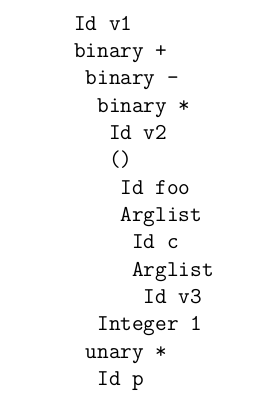
\includegraphics[width=0.4\textwidth]{ast-ex.png}
\end{center}
\section{符号表}
符号表用于存放源程序中与标识符有关的信息,包括标识符名,标识符类型,标识符属性(是否为extern)等。
\subsection{类型表达式}
符号表一个重要的信息域是标识符的类型。一般而言,需要一种类似于类型表达式的数据结构来支持对类型进行相容性判断。这里我们选择可扩充的树型结构来表示源程序中数据的数据类型:
\begin{lstlisting}[language=c]
enum data_type	/* enum for different data types */
{
  Void, Char, Int, Pointer, Array, Function, Typeerror
};

struct typetree
{
	enum data_type type;
	union
	{
		struct typetree * return_type;
		struct typetree * next_parm;
		int size;
	};
	union
	{
	    struct typetree * base_type;
	    struct typetree * parm_list;
	};
};
\end{lstlisting}
对typetree的解读方式如下
\begin{itemize}
\item 如果type的值是Void,Char或者Int,那么说明该类型树表达的是简单类型。
\item 如果type的值是Array,则其基类型由base\_type表示,其长度由size提供。
\item 如果type的值是Pointer,则其基类型由base\_type表示。
\item 如果type的值是Function,则其返回值类型由return\_type表示,而parm\_list则指向了其参数列表的类型树链表。如果一颗类型树是某函数类型的参数,那么其next\_parm指向其在参数列表中的后继。整列表以NULL结束。
\end{itemize}
可以看到,这种类型树的结构可以对MiniC的类型提供完全的支持。事实上即使是C语言全集的数据类型,亦可由这种数据结构表示。
\subsection{组织方式}
考虑到整个编译过程中的需要经常对符号表进行查询,所以我们以散列的方式对符号表进行组织。散列函数采用Unix经典的ELFHash,散列方式为开散列。符号表的构建在语法分析的同时进行。\\
\indent 符号表为每个变量都分配了一个编号(编号方式:前几个编号都是全局变量,函数中的变量从全局变量数开始编号);每个函数都会标记一下参数的起始编号和结束编号;常量字符串也记录在符号表中,插入的时候先为其生成一个名字,然后再存储起来。\\
\indent 于是为了建立符号表到编号、常量字符串的双向链接,就需要在符号表当中放置两个动态数组,分别依下标记录相应变量或字符串常量信息的指针。\\
\indent minic文法支持全局变量和单源文件多函数定义,因此符号表还需要存储与变量作用域有关的信息。我们的处理办法是开辟多个符号表,包括一个全局符号表和多个局部符号表。全局符号表存储全局变量和函数信息;每一个局部符号表对应一个函数,存储函数的局部变量和参数信息等。在对符号表进行查询时,需要首先在当前函数的局部符号表中进行查询,如果查询失败则再在全局符号表中进行查询。
\subsection{构建过程}
现在开始解释构建的详细过程。minic的与变量声明有关的文法如下:
\begin{verbatim}
declaration : modifier type_name var_list ";";
var_list : var_list "," var_item
         | var_item
         ;
\end{verbatim}
可以看到,在词法分析过程中遇到标识符时,并不能立刻得知其类型,需要再经过若干步规约才能得到一个声明序列中所有标识符的基类型,如下面的声明语句:
\begin{lstlisting}[language=c]
  int a, *b, c;
\end{lstlisting}
文法规约的顺序是自右向左,因此在分析到变量名时,变量类型还未归约,因此无法确定变量名的类型。解决的办法是开辟缓冲区对标识符进行暂存,待得到足够信息后再对符号表相应位置进行回填。\\
\indent 另一个比较重要的问题是对字符串常量的处理。之前已经提到,字符串常量在汇编代码中的出现方式与全局变量相似,因此为了方便处理,为每个字符串常量生成一个伪标识符。伪标识符以字符“.”开头,以便区分。
\section{语义检查}
语义检查主要分两部分:类型检查和左值存在性检查。
\subsection{类型检查}
\indent 类型检查的进行基于之前生成的语法树。检查的过程是一个递归的过程:先检查左右子树,得到左右子树的类型,然后根据当前节点的运算类型以及节点左右子树的数据类型在这期间对运算符和运算数的相容性进行检查,并计算当前节点的数据类型,也就是进行隐式类型转换。隐式类型转换的规则与[ANSI]C语言标准完全一致。如果出现类型不相容的情况,则给当前节点赋以Typeerror类型。当对整颗语法树检查完毕后,根据根节点即可得知该语法树对应的表达式中是否有语义错误,同时也得到了所有中间结果的数据类型。
\subsection{左值存在问题}
左值的存在性检查同类型检查在同一过程中进行。根据C语言语义,在进行赋值(=)操作时,要求左操作数拥有左值;在进行引用(\&)操作时,要求操作书拥有左值。拥有左值的变量有以下几种:
\begin{enumerate}
\item 标识符(因字符串常量引入的伪标识符除外)。
\item 解除引用运算(*)得到的结果。
\item 下标运算([])得到的结果。
\end{enumerate}
因此,左值检查的时机是赋值和引用运算,只有被检查的操作数是由上述运算产生时才可通过检查。
\section{中间代码生成}
\subsection{中间代码形式}
minicc的中间代码形式为间接三元式。一般而言,典型的中间代码形式有三元式和四元式两种。这里我们采取间接三元式是为了简化符号表操作,因为四元式需要引入众多临时变量。另外之前已经提到,我们的语法树无法表示控制流。如果采用四元式作为中间代码,那么在实现控制流时就比较繁琐,因为四元式不利于代码顺序的调整。\\
\indent 中间代码生成的结果基本是线性化的抽象语法树,下面给出根据之前的样例语法树生成的三元式序列。
\begin{verbatim}
(0) Arglist c 
(1) Arglist v3 
(2) () foo 
(3) binary * v2 (2) 
(4) binary - (3) 1 
(5) unary * p 
(6) binary + (4) (5) 
(7) = v1 (6) 
\end{verbatim}
三元式的第一部分为运算符,第二和第三部分为运算数。Arglist表示参数传递的操作。中间代码的数据结构如下
\begin{lstlisting}[language=c]
enum triarg_type { IdArg, ImmArg, ExprArg };

struct triarg
{
    enum triarg_type type;
    union
    {
        char* idname;
        int expr; /* use index of the triargexpr, not the address */
        int imme;
        /* used in data flow analyze */
		struct var_list *func_flush_list;
    };
};

struct triargexpr
{
    int index;
    enum operator op;
    int width;
    int stride;
    /* used in data flow analyze */
    struct var_list *actvar_list;
    struct triarg arg1, arg2;
};
\end{lstlisting}
上面的数据结构中大部分信息域完全是三元式自身的信息,也有少量域用来存储数据流分析的一些中间结果。
\indent 在从语法树向三元式转化的过程中,有几个比较重要的问题需要解决。
\subsection{逻辑运算的短路}
第一个问题是逻辑运算的短路问题。根据C语言标准,逻辑运算需要是懒惰的,即在规定的求值顺序下,一旦逻辑表达式的真假可以被确定,则立即停止对表达式剩余部分的求值。要实现这一点,必须在逻辑表达式所对应的三元式中增加额外的跳转判断和跳转代码。\\
\indent 我们采取的解决方案是经典的拉链回填技术,即为每个逻辑表达式维护两个跳转地址链,链中存放需要回填跳转目标的三元式标号。因为在生成逻辑表达式子式对应的三元式,还不知道跳转目标地址,因此需要在链中暂存,至整个表达式分析完毕后再将目标地址回填。下面是一个样例:
\begin{lstlisting}[language=c]
int foo(char * a, int x);
int main()
{
  int a, b, x;
  char * p;
  if(a > 1 || foo(p, x))
  b = 1;
  else
  b = 0;
  return 0;
}
\end{lstlisting}
对应的三元式序列为
\begin{verbatim}
(2) > a 1 
(3) TrueJump (2) (0) 
(4) UncondJump (5) 
(5) Arglist p 
(6) Arglist x 
(7) () foo 
(8) TrueJump (7) (0) 
(9) UncondJump (1) 
(0) = b 1 
(10) UncondJump (11) 
(1) = b 0 
(11) Return 0 
\end{verbatim}
\subsection{逻辑值与算数值之间的转化}
C语言不区分逻辑值和算数值,因此像下面这样的代码是被允许的。
\begin{lstlisting}[language=c]
  int a, b, c;
  // ...
  a = (b < c || a < c) + 1;
\end{lstlisting}
在上面这种情况中,需要对逻辑表达式的结果进行暂存,然后令其参与后续运算。然而在大部分情况下,对于大多数体系结构而言,逻辑表达式的中间结果是不需要暂存的。如何处理这个问题就成了一个难点。这个问题和第一个问题结合在一起时,处理的难度就更大了。\\
\indent 要解决这个问题,需要在表示三元式的数据结构中增加一个域,用于表示当前结果是逻辑值还是算数值。如果在分析语法树某个节点时发现当前运算需要算数值作为操作数,但子树的根节点类型为逻辑值,则需要额外产生算数值的工作。由于三元式中没有显式的临时变量,因此只能引入一种新的操作来表示临时变量。上面表达式翻译成三元式序列的结果是
\begin{verbatim}
(0) < b c 
(1) TrueJump (0) (7) 
(2) UncondJump (3) 
(3) < a c 
(4) TrueJump (3) (7) 
(5) UncondJump (9) 
(6) Temp 
(7) = (6) 1 
(8) UncondJump (10) 
(9) = (6) 0 
(10) binary + (6) 1 
(11) = a (10) 
(12) Return 0 
\end{verbatim}
\subsection{三元式的组织}
我们采用三元式的原因之一,就是三元式利于调度。但是在实现具体的调度机制还是需要一些比较繁复的工作。
比如在实现for循环时,
\begin{lstlisting}
  for_stmt :
  FOR "(" expression ";" expression ";" expression ")" statement ;
\end{lstlisting}
表达式的规约顺序与最终三元式应该的顺序相差甚远。所以当语法分析到达这一步时,需要做一些调整工作。其他控制流的情况类似。
\chapter{编译器后端}
minic后端的任务有:
\begin{enumerate}
\item 根据中间代码进行数据流分析:划分基本块,判断变量的活跃周期。
\item 根据数据流分析的结果进行寄存器分配。
\item 生成目标代码
\end{enumerate}
\newpage
\section{数据流分析}
\subsection{基本块划分及流图化简}
编译器在基本块划分过程中进行了两遍扫描,在这两遍扫描中不仅完成了基本块的划分,还充分利用两遍扫描尽可能地进行了数据处理和代码优化。同时在这一过程中,不仅要进行基本块划分,还要为最后基本块向代码的还原做好准备。下面便对两遍扫描以及之后的流图扫描所实现的功能进行简单的介绍。

\subsubsection{代码的第一遍扫描}
\begin{enumerate}
\item \leavevmode 标记函数中所有可能的入口语句,为第二编扫描中的基本块划分做准备
\item \leavevmode 优化绝对发生的条件跳转为无条件跳转,为第二遍扫描中不可达代码和无用跳转的删除做准备。
  在第一遍扫描中会将所有条件恒为真的TrueJump和条件恒为假的FalseJump改为UncondJump,而将所有条件恒为假的TrueJump和条件恒为真的FalseJump改为Nullop,这样可以防止这样的代码打断基本块,而Nullop在最终生成目标代码时是不产生指令的。例如  向下列代码,在第一遍扫描过程中便会被替换:
\begin{verbatim}
TrueJump 100000 (1)
\end{verbatim}
替换为:
\begin{verbatim}
UncondJump (1)
\end{verbatim}
\item \leavevmode 对三元式数据进行简单分析,为之后的数据流分析、目标代码生成做准备,筛选出函数中所有可能被定值的全局变量,为活跃变量分析中为了保证正确性而对全局变量所做的特殊处理准备。
\item \leavevmode 建立全局变量、局部变量、被引用的临时变量的统一编码,并建立了编码和变量信息之间的双射。对所有三元式编号进行筛选,筛选出被引用的三元式编号做为临时变量与局部变量和全局变量一同进行编码,并建立变量信息与编码之间的双射。这样一方面方便了之后工作中对变量信息的随机查找,另一方面连续的编号也方便寄存器分配时图染色法的实现。
\end{enumerate}
\indent 这一部分使用的数据结构包含所有变量和三元式信息结构体指针的数组,以及一个中间数组map\_bridge,其中中间数组用来建立连续的编号与不连续的临时变量号和局部及全局变量之间的双射。这样虽然需要建立的连续数组的大小是随代码量增加而增加的,但由于本身每一个三元式都要保存在内存中,所以针对每一个三元式建立一个表项是与在三元式中增加一个域相同的,而且这个数组是临时的,在每处理完一个函数后就会被释放掉,所以空尽开销很小。由于是两个数组之间建立的双射,在查找变量信息时可以在常数时间内查到,在一定程度上提高了编译器本身的运行效率。\\
\indent 而且由于整个数据结构都是static的,所以这两个数组对外部文件是不可见的,直接函数接口简洁的实现双射的功能,这样也减少了合作开发时因为诡异的数据结构而产生的协调问题。
\subsubsection{代码的第二遍扫描}
\begin{enumerate}
\item 递归划分基本块,并同时把基本块排列为最有利于数据流分析的深度优先顺序\\
\indent 通过阅读资料,我们了解到,以深度优先的顺序遍历基本块来进行数据流分析,所需的迭代次数是最少的。所以我们便在生成代码的过程中直接把代码看作一个有向图来进行深度优先搜索,在搜索的过程中一方面划分基本块,一方面把基本块以DFS顺序放入数组中,并把尽本块的最后一条语句的跳转地址改为基本块编号,以方便流图到数序代码的还原以及基本块内指令的调度。\\
\indent	在深度优先搜索的过程中,如果发现无条件跳转作为一个基本快的开始语句,则不生成新的基本块,而是继续搜索,并交搜索函数的返回基本块返回,这样便删除了多余的无条件跳转。\\
\indent	在此过程中专门对三地值代码产生过程中产生的一些冗余的代码进行了重点优化:
例如像下列这种代码,由于中间代码产生中不便于调整,所以在基本块划分过程中便对这一类代码进行了重点优化
\begin{lstlisting}[language=c]
  if(a < c)
  {
	;
  }
\end{lstlisting}
\begin{verbatim}
result:
(0)a < c
(1)TrueJump (0) (3)
(2)UncondJump (3)
(3)
\end{verbatim}
在基本块划分过程中,会通过判断条件跳转的两个后继节点是否是相同基本块来进行优化,因为不确定(3)号语句是否还是其它跳转的目标与句,所以无法直接删除跳转,但是可以直接把(1)(2)两条指令合为一条无条件跳转,这样一方面节省了一次条件判断,另一方面该无条件跳转可能会成为唯一能够跳转至后继基本块的跳转,则这种情况下,在尽本块恢复为顺序代码的过程中便会对该类无条件跳转进行删除。
\item 流图的扫描,从基本块恢复为顺序代码,并对代码进行重排序。\\\indent
  对流图进行深度优先搜索,并把基本块还原为重排后的三地址代码存入原来保存三地值代码的结构中。在此过程中,如果发现无条件跳转到的目的地,是该基本块的惟一后继,则对两个基本块进行合并,并删除多余的无条件跳转,这样如果后继基本块是另一基本块的直接后继,则该基本块最后会多产生一条无条件跳转语句,整个程序的无条件跳转数目不变。但是如果该无条件跳转是唯一能够跳到后继基本块的跳转,则此步骤优化了一步无条件跳转。
\end{enumerate}
整个基本块划分过程,一方面充分利用两边扫描,对三元式尽可能地进行了数据分析;一方面又尽可能地对三元式进行了初步的化简,并删除了不可达代码,无用跳转等;另一方面还为数据流分析做好数据准备。
\subsection{数据流分析}
活跃变量分析部分核心在于迭代求解方程和在每个块内求解每一条语句的活跃变量。前者主要涉及数据流分析和集合运算,后者因为与目标代码生成的策略以及优化有关,所以比较繁琐。\\
\indent 首先是集合运算,这就涉及怎样表示集合。我们采用了有序链表来进行集合运算,简称链运算。以c=a并b为例,先将链排排成升序(我们采用的是先把链表复制到临时数组中,快排后在移回来),让NodeA指向a的首节点,NodeB指向b的首节点,如果前者键值大于后者,则将后者键值添加到c中,NodeB后拨;同理,如果前者键值小于后者,则将前者键值添加到c中,NodeA后拨; 如果前者键值等于后者,则将前者键值添加到c中,NodeA和NodeB都后拨。当一条链遍历完的时候,把另一条链所有剩下元素都添加到c中。如此以来就生成了有序的c链。同理交和减运算也都可以做到。这样的复杂度是O(NlogN),但是由于在活跃变量分析中使用链运算结果作为下一次运算的操作链的,所以排序是一劳永逸,单个链运算复杂度就是O(N)。\\
\indent 活跃变量分析的迭代主要涉及:
\begin{displaymath}
	var_{out}[Bi] = +var_{in}[s];s\in NEXT[Bi]
\end{displaymath}
\begin{displaymath}
	var_{in}[Bi] = use[Bi] + (var_{out}[Bi] – def[Bi])
\end{displaymath}
这两个方程。经过观察发现,完成该方程只需要2个链运算函数就可以了:A=A+B、C=A-B。为了方便ud分析的链运算,我们又添加了一个A=A交B的函数。如此以来,这一步完成了。\\
\indent 然后是数据流分析,也就是生成def和use链数组,一开始就是按书上做的定值引用分析,可是等到目标代码生成过程中,我们才发现了很多问题。有一些语句我们必须推迟生成,例如在生成条件跳转语句的时候才会生成它的条件等等。于是有如下注释:
\begin{enumerate}
\item 对于赋值。arg1=arg2
\begin{enumerate}
\item 首先,如果arg1是标号(k)而且k是*p或者a[i],要先分析语句k;(对于指针实体或者数组的定值都只能在赋值语句时生成指令)
\item 分析本条赋值语句。
\end{enumerate}
\item 对于条件跳转。
\begin{enumerate}
\item 首先,如果arg1是一个逻辑条件指令,需要向上看一步,分析三元式arg1;
\item 分析本条条件跳转指令。
\end{enumerate}
\item 对于a+b、a-b、*p、a[i]、+a、-a、\&a以及所有逻辑指令;
\begin{enumerate}
\item 如果这一句话从来没被引用过,没必要生成代码,也就没必要分析;
\item 被引用过则分析本条语句。
\end{enumerate}
\item 对于Funcall,引用分析所有当前函数中可能被定值的全局变量;(进行这一步的原因比较复杂,首先,我们必须保证全局变量和内存的一致性,但是我们又不愿意每次都刷内存,所以就在调用函数和函数返回之前都刷新一遍当前活跃的全局变量。所以我们在每一个可能结束的块末尾和调用函数的一句加入所有可能在当前函数中被定值的全局变量)
\item 其他语句,根据要分析的操作数个数和位置,分以下几种情况:
\begin{enumerate}
\item ++、--
\item Return、Arglist
\item 大立即数
\end{enumerate}
\end{enumerate}
最后是活跃变量生成,这一部分是在块内进行的,从最底下一条语句自底向上分析,上一条语句的活跃变量是在下一条语句的基础上添加add\_list和删除del\_list得到的,其中最底下的语句的活跃变量就是这个块出口处的活跃变量加上这一句的add\_list。生成add\_list和del\_list的方式和上面比较类似。\\
\subsection{指针分析}
由于在机器码生成阶段,对指针所指内存的赋值和引用都可能引起寄存器中数据与内存中数据的不一致,所以需要在对指针所指内存操作前需要通过对所有全局变量和局部变量的load、store来保证寄存器与内存的数据一致性。\\
\indent 于是我们决定使用数据流分析的方法来进行优化,通过数据流分析来确定在数组的每一个引用点上该数组可能指向的变量,从而缩小需要保证寄存器内存一致性的变量的范围,从而减少内存别名操作的开销。\\
\indent 算法设计方面,我们利用利用数据流分析的方法,
	迭代方程:
具体实现时对*、[]、Arglist三种操作进行了分析
\section{寄存器分配}
\subsection{图染色算法}
minic采用图染色法进行寄存器分配。算法流程是
\begin{enumerate}
\item 根据变量的活跃信息构造干涉图。为提高效率,图的结构有两种:三角相邻矩阵和邻接表,它们适用与不同的操作。
\item 搜索干涉图中度数小于可用寄存器数的节点,将其从图中删除并压栈。如果图中已经不存在任何节点,算法转4。如果途中不存在这样的节点,转3。
\item 根据一定策略,将途中某个节点抛出(spill),即将其标记为存储在栈中,并从图中删除。之后算法转2。
\item 从将栈中的节点弹出,分配颜色。
\end{enumerate}
上面算法中删除节点的操作利用相邻矩阵完成更搞笑,而分配颜色的操作利用邻接表完成更高效。算法主体如下:
\begin{lstlisting}[language=c]
  while(left > 0)
  {
    int spill = 1;
    /* igmatrix is the adjacent matrix of the interfer graph */
    get_degree((const char **)igmatrix, n, elem);
    /* sort nodes by degree */
    qsort(elem, n, sizeof(isort_elem), isort_elem_cmp);
    for(i = n - 1; i >= 0; --i)
    {
      if(allocated[elem[i].val])     /* i already allocated */
      continue;
      if(elem[i].key < max_reg)
      {
        /* i can be placed in a reg */
        stack[top++] = elem[i].val;     
        allocated[elem[i].val] = 1;
        delete_node(igmatrix, n, i);
        --left;
        spill = 0;
      }
    }
    if(spill)
    {
      for(i = 0; i < n; ++i)
      {
        if(allocated[elem[i].val])
        continue;
        else /* spill the var having the max degree */
        {
          delete_node(igmatrix, n, elem[i].val);
          (ret.result)[elem[i].val] = -1;
          allocated[elem[i].val] = 1;
          --left;
          break;
        }
      }
    }
  }
\end{lstlisting}
\subsection{抛出(spill)策略}
算法中的抛出(spill)策略比较简单,每次都选择产生干涉最多的变量进行抛出。由于UniCore2体系结构是通用寄存器结构,寄存器数目较多,所以即使是这样简单的寄存器分配策略也可以有很好的效果。
\subsection{寄存器的使用}
minicc的寄存器分配算法是一个通用的算法,像可用寄存器数这样的信息是以参数的形式给出的,因此算法本身与体系结构无关。相应地,算法给出的分配结果也不对应机器级别的寄存器号,而是需要再做一次映射。这么做的好处是算法实现简单,且只要改变映射关系就可以调整对寄存器的使用策略。\\
minicc对寄存器的使用基本遵守UniCore2的ABI规范,但还是有一些不同。比如静态基址寄存器和过程间寄存器在实习的要求框架内并无特殊用途,因此我们也将其视为普通的可用寄存器。
\section{机器码生成}
目标代码生成部分比较复杂,因为每个操作数,除了立即数,都有可能在内存或者在寄存器,后者可以直接使用,前者需要申请临时寄存器——有的时候立即数也要申请临时寄存器。这样以来情况就比较复杂了。再加上我们试图在生成时候就尽量做到指令最简。
\subsection{数据结构}
如我们一往之风格,在设计机器码表示的时候首先考虑的是数据结构的规整性。
\begin{lstlisting}[language=c]
enum mach_arg_type { Unused, Mach_Reg, Mach_Imm, Mach_Label};
struct mach_arg
{
    enum mach_arg_type type;//when not used, use -1
    union
    {
        int reg;
		int imme;
		char * label;
    };
};

enum mach_op_type { /* ... */ };
enum dp_op_type { /* ... */ };
enum cmp_op_type { /* ... */};
enum mem_op_type { /* ... */};
enum branch_op_type { /* ... */ };
enum condition_type { /* ... */ };
enum shift_type { /* ... */ };
enum index_type { /* pre, post... */ }; 

struct mach_code//mach means machine
{
	enum mach_op_type op_type;
	union
	{
		char * label;
		enum dp_op_type dp_op;
		enum cmp_op_type cmp_op;
		enum mem_op_type mem_op;
		enum branch_op_type branch_op;
	};
	union
	{
		int dest; //only reg
		char * dest_label;//for cond jump
	};
	union
	{
		struct mach_arg arg1;
        /* used in condition-jump */
		enum condition_type cond;
	};		
	struct mach_arg arg2;
	uint32_t arg3; /* can only be constant */
	union
	{
		char link;
		char offset;
	};
	enum index_type indexed;
	char optimize;
	enum shift_type shift;
};
\end{lstlisting}
\subsection{赋值翻译举例}
比如arg1 = arg2翻译步骤:
\begin{enumerate}
\item 如果当前arg1不是活跃变量,不进行此赋值;
\item 赋值。
\begin{enumerate}
\item 赋值操作
\begin{enumerate}
\item arg1和arg2是寄存器,或者arg1是寄存器而arg2是立即数,MOV;
\item arg1是寄存器,arg2是内存,load;
\item arg1是内存,arg2是寄存器,store;
\item arg1是内存,arg2是立即数,申请临时寄存器,存入arg2,然后store;
\item arg1和arg2都是内存,先将arg2导入临时寄存器,然后将临时寄存器的值存入内存。
\end{enumerate}
\item 如果arg1是三元式编号,还要看一下它对应的三元式是否是*p或者a[i],如果是的话,还要对内存操作。
\end{enumerate}
\item 指针相关操作。
\begin{enumerate}
\item 如果arg1是(*arg)的形式,需要把(*arg)可能指向的所有变量对应的寄存器都写入内存(假如它当前是活跃的)。
\end{enumerate}
\end{enumerate}

\subsection{大立即数产生算法}
UniCore2指令系统采用定长编码方式,指令长度为4个字节,因此无法直接使用较大的立即数作为指令操作数。与立即数有关的操作指令格式如下
\begin{center}
  \begin{tabular}{ccccc}
    8 bits & 5 bits & 5 bits & 5 bits & 9bits \\
    \hline
    operation \cellcolor{rgb:red,2;green,1;yellow,1}& rs\cellcolor{rgb:red,0;green,1;yellow,1} & rd\cellcolor{rgb:red,0;green,0;blue,1} & shift\_imm \cellcolor[gray]{.9}& imm\_operand \cellcolor{rgb:red,5;green,0;yellow,0}\\
    \hline
  \end{tabular}
\end{center}
对于这样格式的指令,第二个源操作是由9位的imm\_operand经过shift\_imm次循环右移得到的32位数。根据这个特点,所有立即数都可以通过将其拆分为若干部分,然后做或位运算得到。由于立即数编码中的0是无需产生的,因此可以跳过立即数中连续的0。\\
\indent 下面是描述minicc产生一般性的大立即数的算法的代码:
\begin{lstlisting}[language=c]
int lsb = 0; /* least significant bit position*/
int temp;
while(((target >> lsb) & 1) == 0)
  ++lsb;
/* rotate shift right by 32-lsb bits */
temp = (target >> lsb) & 0x1ff;
temp = (temp << lsb) | (temp >> (32 - lsb));

result = temp; /* move instruction */
lsb += 9;
while(lsb < 32)
{
  while(lsb < 32 && ((target >> lsb) & 1) == 0)
    ++lsb;
  if(lsb >= 32)
    break;
  temp = (target >> lsb) & 0x1ff;
  /* rotate shift right by 32-lsb bits */
  temp = temp << lsb | (temp >> (32 - lsb));
  result |= temp;               /* or instruction*/
  lsb += 9;
}
\end{lstlisting}
利用上面的算法,可以把立即数的产生控制在4条指令之内。\\
\indent 在判断大立即数时,将目标都视为无符号数。但在实际情况中,程序员用到绝对值较小的负数的情况还是较多的。对于-512到-1的立即数,可以通过一条not指令得到,无需采用上面算法。\\
\indent 下面给出一个产生大立即数{\color{red}1111 11110000 0000 0001 0100 1111 0000}的样例:
\begin{figure}[H]
\centering
\begin{tabular}{|l|l|}
\hline
指令序列 & 中间结果\\
\hline
 mov r, \#335<>28  & 0000 0000 0000 0000 000{\color{red}1 0100 1111} 0000 \\
\hline
or r, r, \#255<>8  & {\color{red}1111 1111} 0000 0000 0001 0100 1111 0000 \\
\hline
\end{tabular}
\end{figure}
\chapter{编译优化}
在保证编译器正确性的基础上,我们额外做了一些编译优化工作。事实上在实现编译器后端的时候,我们就已经考虑了很多效率方面的问题,诸多细节方面的优化已经融入实现中。这一部分主要介绍三项比较有代表性的优化工作。
\newpage
\section{指令调度}
之前已经提到,minic是需要与MiniSim模拟器协同工作的。因此,根据MiniSim的实现,可以通过一些指令调度策略来提高模拟的性能。\\
\indent MiniSim模拟五级流水结构,因此由于数据相关而产生的加载互锁是性能的一大瓶颈,我们的优化也主要针对这一情况。minicc通过将产生数据相关的load指令提前,可以有效减少加载互锁发生的次数。这里指令调度主要通过窥孔的方式实现。\\
\indent 在目标代码生成后,按序对目标代码进行扫描,如果load语句与紧跟的一条语句存在数据相关,则把这两条这令看作一个整体,生成两个集合:定值寄存器集和引用寄存器集;之后向上看一条代码,如果该条代码的有可能修改的寄存器在引用寄存器集中或该条代码所需引用的寄存器在定植寄存器集中,则该条指令无法调度,把该条指令有可能修改的寄存器加入定值寄存器集,把可能引用的寄存器加入引用寄存器集中,继续看上一条代码。\\
\indent	一旦发现与整个定植寄存器集和引用寄存器集不相关的指令便可以调度。其中如果遇到跳转指令或标号,说明基本块已到上界,停止调度;如果遇到stw指令,因为在目标代码阶段无法确定改指令修改的是否是load引用的内存,所以无法确定是否有数据相关,所以直接默认存在数据相关,把改制令纳入定植寄存器集及引用寄存器集中,继续看上一条指令。可以通过设定指令窗口大小,来设置最大向上看的步数,不过一般基本块都不会太大。
\section{赋值操作与对应产生右值的操作的合并}
由于在中间代码生成阶段使用的是三元式,所以在充分利用三寄存器操作的指令上出现了一些困难,例如一个赋值操作:
\begin{verbatim}
	a = b + c
	需要两条三元式
	(1) + b c
	(2) = a (1)
\end{verbatim}
而这显然在生成代码时是浪费的,但是在目标代码生成阶段直接生成一条代码有一定的麻烦,所以我们在中间代码分析阶段对对应的指令进行了标记,并在生成的有可能优化的目标代码中加入了optimize标记,所以在窥孔阶段,一旦发现该条指令是可有化的(optimize == 1),则看下一条指令是否是mov指令,如果是则对两条指令进行合并。
\section{指令强度优化}
这项优化针对的是高强度运算。在MiniC的范围内,这项优化主要针对的是乘法,即一个乘数是立即数时可以将乘法转化为移位和加减运算。由于UniCore2体系结构中整点乘法只比普通ALU运算多耗一个周期,所以只有乘数是2的幂或者和2的幂相差1才可以优化:
\begin{figure}[H]
\centering
\begin{tabular}{|l|l|}
\hline
	乘数是$2^i$		& mov reg, reg << i\\
\hline
	乘数是$2^i – 1$	& rsub reg, reg, reg << i\\
\hline
	乘数是$2^i + 1$	& add reg, reg, reg << i\\
\hline
\end{tabular}
\end{figure}
\section{效率测试}
为了测试minicc的编译功效,我们编写了两个基准程序:快速排序和冒泡排序。测试平台为MiniSim模拟器,Cahce策略为LRU、Write-back。
\begin{enumerate}
\item 快速排序
\leavevmode
\begin{lstlisting}[language=c]
/* quicksort.c */
extern int printline_int(int x);
extern int a[10000];
void quicksort(int * beg, int * end)
{ 
    int * left;
    int * right;
    int temp;
	int out_loop;
	
	left = beg;
	right = end;
	temp = *left;
	
	if(end <= beg)
        return;
    while(left < right)
    {
		out_loop = 1;
        while(left < right && out_loop == 1)
        {
            if(*right < temp)
            {
                *left = *right;
				++left;
				out_loop = 0;
            }
            else
                --right;
        }
        while(left < right && out_loop == 0)
        {    
            if(*left > temp)
            {
                *right = *left;
                --right;
				out_loop = 1;
			}
            else
                ++left;
        }   
    }
    *left = temp;
    quicksort(beg, left - 1);
    quicksort(left + 1, end);
    return;
}

int main()
{
    int j, temp;
    quicksort(a, a + 9999);
    for(j = 0; j < 10000; ++j)
        printline_int(a[j]);
    return;
}
\end{lstlisting}
\begin{figure}[H]
\centering
\begin{tabular}{|l|c|c|c|c|c|}
\hline
编译器 & 周期数 & 动态指令数 & nop & 访存次数 & Cache失效 \\ 
\hline
gcc   & 16429875 & 12637758 & 6934740 &  6362459 &  2965\\
\hline
gcc -O1 & 7551253 & 6836257 &  3637868 &  887412 &  2242 \\
\hline
gcc -O2 & 7723437 & 7020307 &  3467600 &  824195 & 1704 \\
\hline
minicc & 7840103 & 7073730 & 3741101 & 924375 & 2943 \\
\hline
\end{tabular}
\end{figure}
\item 冒泡排序
\begin{lstlisting}[language=c]
/* bubble sort */
extern int printline_int(int x);
extern int a[10000];

int main()
{
    int i, j, temp;
    for(i = 10000; i >0; --i)
    {
        for(j = 0; j < i; ++j)
            if(a[j] > a[j+1])
            {
                temp = a[j+1];
                a[j+1] = a[j];
                a[j] = temp;
            }
    }
    for(j = 0; j < 10000; ++j)
        printline_int(a[j]);
    return 0;
}
\end{lstlisting}
\begin{figure}[H]
\centering
\begin{tabular}{|l|c|c|c|c|c|}
\hline
编译器 & 周期数 & 动态指令数 & nop & 访存次数 & Cache失效 \\ 
\hline
gcc   & 1792650583 & 1299872441 & 661707908 & 870352582 & 844095 \\
\hline
gcc -O1 & 460235557 & 403026442 & 150065009 & 152891428 & 800457 \\
\hline
gcc -O2 & 460292123 & 453025691 & 100060007 & 152915680 & 806270 \\
\hline
minicc & 719047444 & 635294973 &  252971423 & 205792833 & 811307 \\
\hline
\end{tabular}
\end{figure}
\end{enumerate}
\chapter{使用说明}
minicc接受的参数格式为:
\begin{center}
  minicc [OPTIONS...] SOURCE\_FILE
\end{center}
可选的参数有:
\begin{itemize}
\item -a 打印编译中间结果:语法树
\item -t 打印编译中间结果:三元式
\item -d 打印调试相关信息:基本块、活跃变量、寄存器分配信息。
\end{itemize}
如果输入文件以.c为后缀,则minicc输出前缀相同,以.s为后缀之文件。如果输入文件不以.c为后缀,则输出文件名为输入文件名追加.s后缀。
\end{document}
